\chapter {معماری  موتور بازی‌سازی آنریل}
در این فصل ابتدا به معماری موتور آنریل پرداخته شده و پس از آن درباره‌ی ابزار‌هایی که این انجین در اختیار ما می‌گذارد صحبت می شود.

\section {\lr{ UObject} \, و \, \lr{ Actors}}

کلاس پایه برای تمامی کلاس‌های دیگر در موتور آنریل
\lr{UObject}
است.
‌شئ‌ها
\LTRfootnote{Objects}
‌نمونه‌هایی از کلاس‌هایی هستند که از 
\lr{UObject}
ها ارث می‌برند.
بازیگران
\LTRfootnote{Actors}
نمونه‌هایی از کلاس‌هایی هستند که از.
\lr{AActor}
ارث برده اند.
کلاس 
\lr{AActor}
کلاس پایه برای تمامی اشیائی است که می‌توانند در جهان بازی قرار گیرند.
به صورت کلی، بازیگران را می‌توان به عنوان یک کل یا موجودیت در نظر گرفت و اشیاء را قطعات تخصصی‌ای درنظر گرفت که در این موجودیت به کار می‌روند
که به آن‌ها جزء 
\LTRfootnote{Component}
می‌گویند.
بنابراین اجزاء یک نوع خاصی از اشیاء هستند که بازیگران می‌توانند آن‌ها را به عنوان یک زیر‌شئ
\LTRfootnote{sub-object}
به خود متصل کنند.

به عنوان مثال اگر یک ماشین را درنظر بگیریم. ماشین به عنوان یک موجودیت کلی به عنوان بازیگر درنظر گرفته می‌شود. در صورتی که قسمت‌های مختلف این ماشین مانند درِ ماشین یا چرخ ماشین اجزای آن ماشین درنظر گرفته می‌شوند. در ادامه این مثال، اگر کاربر قرار باشد که این ماشین را کنترل کند، یک جزء دیگر می‌تواند مسئولیت تغییر سرعت و جهت ماشین بر اساس ورودی کاربر را داشته باشد.
\cite{UnrealEngineArchitecture, UnrealEngineComponents}

\section{\lr{Components}}
همانطور که گفته‌شد، اجزاء نوع خاصی از اشیاء هستند که بازیگران می‌توانند به عنوان اشیاء فرعی به خود متصل کنند.
کلاس پایه برای تمامی اجزاء، کلاس
\lr{UActorComponent}
است. از آنجایی که استفاده از اجزاء تنها راه ممکن برای پرداخت
\LTRfootnote{Render}
مش‌ها
\LTRfootnote{Meshes}
، تصاویر
،پخش صداو درواقع هرچیزی که بازیکن هنگام بازی در جهان مشاهده یا تعامل می‌کنند هستند، بنابراین در نهایت از انواعی از این نوع اجزاء در توسعه‌ی بازی استفاده می‌شود.

برای ساخت اجزاء، چند کلاس اصلی وجود دارد که در هنگام ایجاد اجزاء باید به آن توجه کرد.

\begin{itemize}
	\item اجزای بازیگر\LTRfootnote{ActorComponent}: این کلاس بیشتر برای رفتارهای انتزاعی مانند حرکت، مدیریت موجودی یا ویژگی و سایر مفاهیم غیرفیزیکی مفید هستند. این نوع از اجزاء هیچ گونه مکان فیزیکی یا چرخشی در جهان ندارد.
	\item اجزای صحنه \LTRfootnote{SceneComponent}: این کلاس فرزند کلاس اجزای بازیگر است و از رفتار‌های مبتنی بر مکان پشتیبانی می‌کند که به نمایش هندسی نیاز ندارند. این کلاس می‌تواند شامل بازوهای فنری، دوربین‌ها، نیروهای فیزیک و حتی صدا شود.
	\item اجزای اولیه \LTRfootnote{Primitive Components}: این کلاس فرزند کلاس اجزای صحنه است. درواقع این کلاس همان کلاس اجزای صحنه، همراه با نمایش هندسی است که عموما برای نمایش عناصر بصری و برخورد
	\LTRfootnote{collide}
	یا همپوشانی
	\LTRfootnote{overlap}
	با اشیاء فیزیکی استفاده می‌شود. این کلاس می‌تواند شامل مش‌های استاتیک
	\LTRfootnote{static mesh}
	یا اسکلتی
	\LTRfootnote{skeletal mesh}
	، اسپرایت‌ها یا بیلبورد‌ها، سیستم‌های ذرات
	\LTRfootnote{particle systems}
	و همچنین حجم برخورد
	\LTRfootnote{collision volumes}
	جعبه، کپسول و کره شود.
\end{itemize}

\cite{UnrealEngineComponents}

\begin{figure}[ht]
	%\centerline{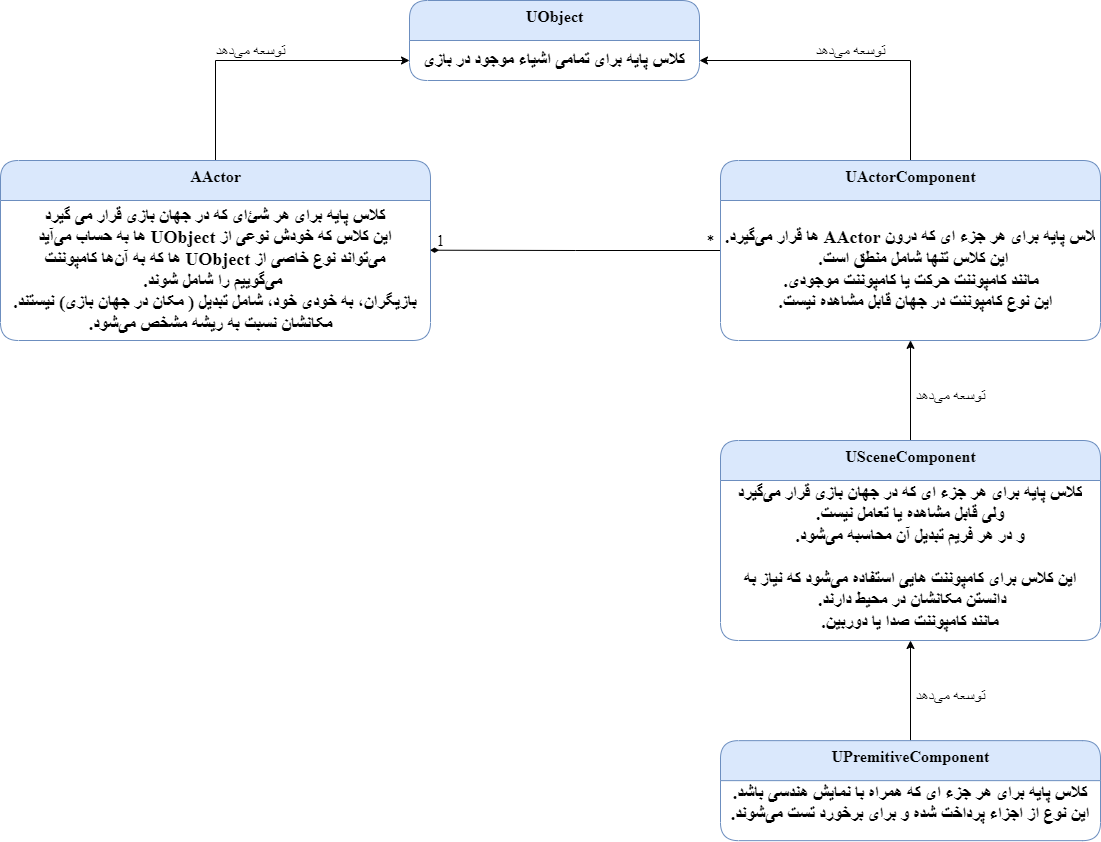
\includegraphics[scale=0.5]{Figures/Ch2/UnrealEngineBasicClassesUML.png}}
	\centerline{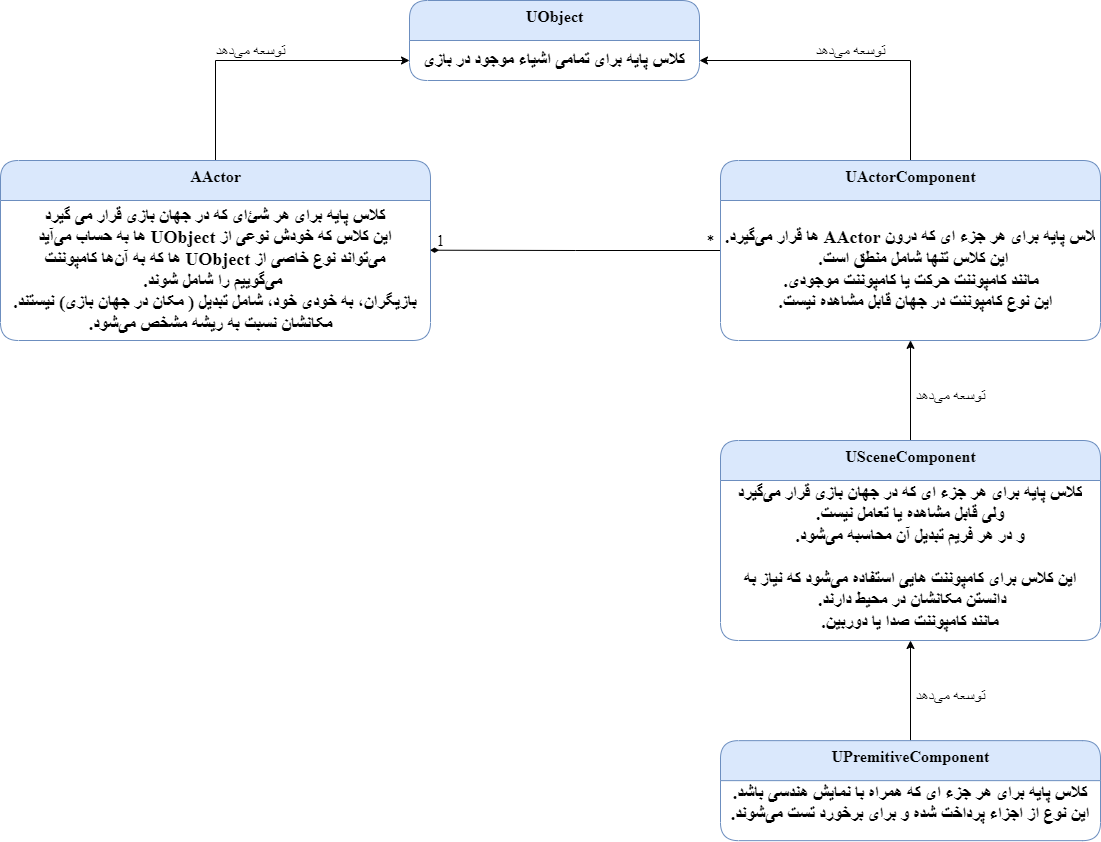
\includegraphics[width=\textwidth,height=\textheight,keepaspectratio]{Figures/Ch2/UnrealEngineBasicClassesUML.png}}

	\caption{تصویر \lr{UML} کلاس‌های پایه‌ی موتور‌ بازی‌سازی آنریل}
	\label{fig:UnrealEngineBasicClassesUML}
  \end{figure}
  